\documentclass[english]{ccdconf}
\begin{document}


\title{Template for Preparation of Papers for Chinese Control and Decision Conference}
\author{Jiang Liu\aref{amss,amss1,hit2}, Meihua Zhong\aref{amss,hit},
      Huanhuan Chen\aref{hit}}

\affiliation[amss]{School of Information Science and Engineering,
Northeastern University, Shenyang, 110004
        \email{aaa@mail.neu.edu.cn}}
\affiliation[hit]{Harbin Institute of Technology, Harbin 150001,
China
        \email{bbb@163.com}}
\affiliation[amss1]{School of Information Science and Engineering,
Northeastern University, Shenyang, 110004
        \email{aaa@mail.neu.edu.cn}}
\affiliation[hit2]{Harbin Institute of Technology, Harbin 150001,
China
        \email{bbb@163.com}}

\maketitle

\begin{abstract}
These instructions give you basic guidelines for preparing papers
for Chinese Control and Decision Conference . Note that ``Abstract''
and ``Key Words'' are bold.
\end{abstract}

\keywords{Paper, Instruction, Chinese Control and Decision
Conference }

\footnotetext{This work is supported by National Nature Science
Foundation under Grant ********.}

\section{INTRODUCTION}

These are instructions for authors typesetting for the Chinese
Control and Decision Conference (CCDC). This document has been
prepared using the required format. \textbf{Please use this document
as a ``template'' to prepare your manuscript. For submission
guidelines, follow instructions on paper submission system as well
as the Conference website.}

The paper is to be written in two-column format and be right and left
justified. The column width should be 82.5mm. The gap between the two
columns should be 7mm.

\subsection{Instructions for Authors}

In order for the proceedings to be ready for distribution at the
conference, an electronic copy (PDF format) of the final version of
your paper must be submitted via CCDC Paper Management System via
\URL{http://www.ccdc.neu.edu.cn/}. Please follow the submission
instructions shown on the web site.

\section{FORMATTING INSTRUCTIONS}

\LaTeXe{} Authors: please try to use the paragraph styles contained
in this document.

\subsection{Length}

The maximum allowed number of pages is 6.

\subsection{Page/Font Settings}

It is strongly recommended that prospective authors download
suitable style file for use with \LaTeX{} and templates for use with
MS Word.

Style files and templates provided here have been created to ensure
that margin requirement is adequately met. If, for some reason, you
are not able to use provided templates or style files, please
observe the following margins and font settings strictly.

\begin{table}
  \centering
  \caption{Page Margins}
  \label{tab1}
  \begin{tabular}{l|l}
    \hhline
    Paper Size          & (21$\times$29.7)cm \\ \hline
    Top Margin (1st page)   & 3.5cm \\ \hline
    Top Margin (rest)   & 2cm \\ \hline
    Left Margin         & 1.9cm \\ \hline
    Right Margin        & 1.9cm \\ \hline
    Bottom Margin       & 2.7cm \\ \hline
    Text Width          & 17.2cm \\ \hline
    Text Height         & 25cm \\ \hline
    Column Width        & 8.25cm \\ \hline
    Column Separation       & 0.7cm \\
    \hhline
  \end{tabular}
\end{table}

\begin{table}
  \centering
  \caption{Font Settings}
  \label{tab2}
  \begin{tabular}{c|c}
    \hhline
    Title           & Times New Roman, 16pt,bold \\ \hline
    Author List         & Times New Roman, 11pt \\ \hline
    Authors�� Address       & 9pt \\ \hline
    Abstract, Key Words     & 9pt \\ \hline
    Section Titles      & 11pt,bold \\ \hline
    Subsection Titles       & 10pt,bold \\ \hline
    Normal Text         & 10pt \\ \hline
    Table/Figure Captions   & 9pt \\ \hline
    References, Footnotes   & 8pt \\
    \hhline
  \end{tabular}
\end{table}

\subsection{Section and Subsection Headings}

Number section and subsection headings consecutively in Arabic numbers and
type them in bold. Avoid using too many capital letters. If any further
subdivision of a subsection is needed the titles should be 10 point and
flushed left.

\subsection{Main Text}

Use Times New Roman with font size 10 point for text (character
size). Paragraphs are separated by 6 point and with no indentation.
You may type on plain white A4 paper. Typing area should not exceed
172mm${}\times{}$250mm. The text should be prepared with a double
column format and single line spacing.

\subsection{Tables}

All tables must be centered in the column and numbered consecutively
(in Arabic numbers). Table headings should be placed above the table.
Place tables as close as possible to where they are mentioned in the
main text (see Table~\ref{tab1} and Table~\ref{tab2}).

\subsection{Figures}

All illustrations should be original drawings or photographic prints of
originals.  Photographs should be glossy prints. Photocopies are often
not good enough and should be avoided.  All illustrations must be numbered
consecutively, using Arabic numbers.  Center figure captions beneath the
figure (see Figure~\ref{fig1}). If possible, do not assemble figures at the
back of your article, but place them as close as possible to where they are
mentioned in the main text. No part of a figure should go beyond the typing
area. Captions should appear below graphical objects, as in Figure~\ref{fig1}.

\begin{figure}
  \centering
  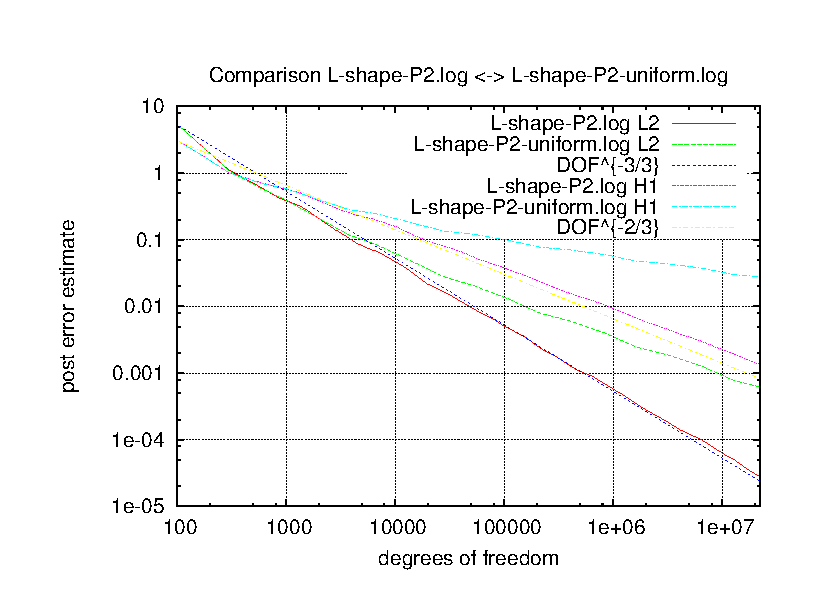
\includegraphics[width=\hsize]{fig1.eps}
  \caption{The Caption}
  \label{fig1}
\end{figure}

Color and grayscale figures should be prepared with 400 dpi
resolution and  saved with no compression, monochrome figure should
be prepared with 600 dpi resolution and saved with no compression.

\subsection{Mathematical Formulas}

Mathematical formulas should be roughly centered and have to be numbered
as formula~(\ref{eq1}).
\begin{equation}
  \label{eq1}
  \lambda_{1,2} = 0.5 \left[\, c_{11} + c_{12}
            \sqrt{(c_{11} + c_{12})^2 + 4 c_{12} c_{21}} \,\right]
\end{equation}

\subsection{References}

Number citations consecutively in square brackets \cite{bib1}. The
sentence punctuation follows the brackets \cite{bib3}. Please note
that the references at the end of this document are in the preferred
referencing style. Give all authors's names; do not use ``et al.''
unless there are six authors or more. Use a space after authors'
initials.

%
% Note: place a \balance command somewhere within the left column of the
% last page will balance the two columns on the last page.
%
\balance

\section{CHECKLIST}

\begin{itemize}
  \item Do not end a page with a section or subsection heading.
  \item Do not include page numbers in the text.
  \item Large figures, tables and mathematical equations may span both columns.
  \item To balance the two columns on the last page, place the command
    \verb|\balance| somewhere in the text of what would be the first
    column of the last page without balanced columns.
  \item If you have to plug a large formula, table, etc.,  which needs a cross
  column space, you must add option \verb|usemulticol| into the
  commend \verb|\documentclass|, then use the commend
  \verb|\singlecolumn{content}| to input cross column contents.


\end{itemize}

\section{PAPER SUBMISSION}

After proofreading your paper, it (PDF formats) must be submitted
via \URL{http://www.ccdc.neu.edu.cn/}.


\begin{thebibliography}{0}

\bibitem{bib1}D. Z. Cheng, Controllability of switched  bilinear systems, IEEE
Trans. on Automatic Control, Vol.50, No.4, 511-515, 2005.
%----------the format for published papers-----------------

\bibitem{bib3} H. Poor, An Introduction to Signal Detection and
Estimation,   New York: Springer-Verlag, Chap. 4, 1985.
%--------- the format for books-------------------------

\bibitem{bib4} B. Smith, An approach to graphs of linear forms, accepted.

\end{thebibliography}

\end{document}
